% -*- latex -*-

\chapter{Worklets}
\label{chap:Worklets}

\index{worklet|(}

The simplest way to implement an algorithm in VTK-m is to create a
\keyterm{worklet}. A worklet is fundamentally a functor that operates on an
element of data. Thus, it is a \textcode{class} or \textcode{struct} that
has an overloaded parenthesis operator (which must be declared
\textcode{const} for thread safety). However, worklets are also embedded
with a significant amount of metadata on how the data should be managed and
how the execution should be structured. This chapter explains the basic
mechanics of defining and using worklets.


\section{Worklet Types}
\label{sec:WorkletTypes}

\index{worklet~types|(}

Different operations in visualization can have different data access
patterns, perform different execution flow, and require different
provisions. VTK-m manages these different accesses, execution, and
provisions by grouping visualization algorithms into common classes of
operation and supporting each class with its own worklet type.

Each worklet type has a generic superclass that worklets of that particular
type must inherit. This makes the type of the worklet easy to identify. The
following list describes each worklet type provided by VTK-m and the
superclass that supports it. Details on how to create worklets of each type
are given in Section~\ref{sec:CreatingWorkletsOfType}. It is also possible
to create new worklet types in VTK-m. This is an advanced topic covered in
Chapter~\ref{chap:AdvancedWorklets}.

\begin{description}
\item[Field Map] \index{worklet~types!field~map} \index{field~map~worklet}
  A worklet deriving \vtkmworklet{WorkletMapField} performs a basic mapping
  operation that applies a function (the operator in the worklet) on all
  the field values at a single point or cell and creates a new field value
  at that same location. Although the intention is to operate on some
  variable over a mesh, a \textidentifier{WorkletMapField} may actually be
  applied to any array. Thus, a field map can be used as a basic
  \index{map}map operation.

\item[Topology Map] \index{worklet~types!topology~map}
  \index{topology~map~worklet} A worklet deriving
  \vtkmworklet{WorkletMapTopology} or one of its sibling classes performs a
  mapping operation that applies a function (the operator in the worklet)
  on all elements of a particular type (such as points or cells) and
  creates a new field for those elements. The basic operation is similar to
  a field map except that in addition to access fields being mapped on, the
  worklet operation also has access to incident fields.

  There are multiple convenience classes available for the most common
  types of topology mapping. \index{worklet~types!point~to~cell}
  \index{point~to~cell~worklet} \vtkmworklet{WorkletMapPointToCell} calls
  the worklet operation for each cell and makes every incident point
  available. This type of map also has access to cell structures and can
  interpolate point fields.
  %% \index{worklet~types!cell~to~point}
  %% \index{cell~to~point~worklet} \vtkmworklet{WorkletMapCellToPoint} calls
  %% the worklet operation for each point and makes every incident cell
  %% available.
\end{description}

\index{worklet~types|)}


\section{Dispatchers}
\label{sec:Dispatchers}

\index{dispatcher|(}

Worklets, both those provided by VTK-m as listed in
Section~\ref{sec:ProvidedWorklets} and ones created by a user as described
in Section~\ref{sec:CreatingWorklets}, are instantiated in the control
environment and run in the execution environment. This means that the
control environment must have a means to \index{invoke}\keyterm{invoke}
worklets that start running in the execution environment.

This invocation is done through a set of
\index{dispatcher}\keyterm{dispatcher} objects. A dispatcher object is an
object in the control environment that has an instance of a worklet and can
invoke that worklet with a set of arguments. There are multiple types of
dispatcher objects, each corresponding to a type of worklet object. All
dispatcher objects have at least two template parameters: the worklet class
being invoked, which is always the first argument, and the device adapter
tag, which is always the last argument and will be set to the default
device adapter if not specified.

All dispatcher classes have a method named \textcode{Invoke} that launches
the worklet in the execution environment.  The arguments to
\textcode{Invoke} must match those expected by the worklet, which is
specified by something called a \keyterm{control signature}. The expected
arguments for worklets provided by VTK-m are documented in
Section~\ref{sec:ProvidedWorklets}. Also, for any worklet, the
\textcode{Invoke} arguments can be gleaned from the control signature,
which is described in Section~\ref{sec:ControlSignature}.

The following is a list of the dispatchers defined in VTK-m. The
dispatcher classes correspond to the list of worklet types specified in
Section~\ref{sec:WorkletTypes}. Many examples of using these dispatchers
are provided in Section~\ref{sec:ProvidedWorklets}.

\begin{description}
\item[\vtkmworklet{DispatcherMapField}] The dispatcher used in conjunction
  with a worklet that subclasses \vtkmworklet{WorkletMapField}. The
  dispatcher class has two template arguments: the worklet type and the
  device adapter (optional).
\item[\vtkmworklet{DispatcherMapTopology}] The dispatcher used in
  conjunction with a worklet that subclasses
  \vtkmworklet{WorkletMapTopology} or one of its sibling classes (such as
  \vtkmworklet{WorkletMapPointToCell}). The dispatcher class has two
  template arguments: the worklet type and the device adapter (optional).
%% \item[\daxcont{DispatcherMapCell}] The dispatcher used in conjunction with
%%   a worklet that subclasses \dax{WorkletMapCell}. The class has two
%%   template arguments: the worklet type and the device adapter (optional).
%% \item[\daxcont{DispatcherGenerateTopology}] The dispatcher used in
%%   conjunction with a worklet that subclasses
%%   \dax{WorkletGenerateTopology}. The class has three template arguments: the
%%   worklet type, the type of array handle containing the count of the number
%%   of cells being generated (optional), and the device adapter
%%   (optional). The default type of the count array handle is
%%   \daxcont{ArrayHandle}\textcode{<}\dax{Id}\textcode{>}. An instance of the
%%   count array handle must be provided in the constructor of
%%   \daxcont{DispatcherGenerateTopology}.
%% \item[\daxcont{DispatcherInterpolatedCell}] The dispatcher used in
%%   conjunction with a worklet that subclasses
%%   \dax{WorkletInterpolatedCell}. The class has three template arguments: the
%%   worklet type, the type of array handle containing the count of the number
%%   of cells being generated (optional), and the device adapter
%%   (optional). The default type of the count array handle is
%%   \daxcont{ArrayHandle}\textcode{<}\dax{Id}\textcode{>}. An instance of the
%%   count array handle must be provided in the constructor of
%%   \daxcont{DispatcherInterpolatedCell}.
%% \item[\daxcont{DispatcherGenerateKeysValues}] The dispatcher used in
%%   conjunction with a worklet that subclasses
%%   \dax{WorkletGenerateKeysValues}. The class has three template arguments:
%%   the worklet type, the type of array handle containing the count of the
%%   number of key-values being generated (optional), and the device adapter
%%   (optional). The default type of the count array handle is
%%   \daxcont{ArrayHandle}\textcode{<}\dax{Id}\textcode{>}. An instance of the
%%   count array handle must be provided in the constructor of
%%   \daxcont{DispatcherGenerateKeysValues}.
%% \item[\daxcont{DispatcherReduceKeysValues}] The dispatcher used in
%%   conjunction with a worklet that subclasses
%%   \dax{WorkletReduceKeysValues}. The class has three template arguments:
%%   the worklet type, the type of array handle containing the keys
%%   (optional), and the device adapter (optional). The default type of the
%%   key array handle is
%%   \daxcont{ArrayHandle}\textcode{<}\dax{Id}\textcode{>}. An instance of the
%%   key array handle must be provided in the constructor of
%%   \daxcont{DispatcherReduceKeysValues}.
\end{description}

\index{dispatcher|)}

\section{Provided Worklets}
\label{sec:ProvidedWorklets}

\fix{Write this once some worklets are provided.}


\section{Creating Worklets}
\label{sec:CreatingWorklets}

\index{worklet!creating|(}

A worklet is created by implementing a \textcode{class} or
\textcode{struct} with the following features.

\begin{enumerate}
\item The class must contain a \controlsignature \textcode{typedef}, which
  specifies what arguments are expected when invoking the class with a
  dispatcher in the control environment.
\item The class must contain an \executionsignature \textcode{typedef},
  which specifies how the data gets passed from the arguments in the
  control environment to the worklet running in the execution environment.
\item The class must contain an \inputdomain \textcode{typedef}, which
  identifies which input parameter defines the input domain of the data.
\item The class may define a scatter operation to override a 1:1 mapping
  from input to output.
\item The class must contain an overload of the parenthesis operator, which
  is the method that is executed in the execution environment.
\item The class must publicly inherit from a base worklet class that
  specifies the type of operation being performed.
\end{enumerate}

Figure~\ref{fig:WorkletExampleAnnotated} demonstrates all of the required
components of a worklet.

%% \pagebreak
%% \begin{vtkmexample}{Example Code for Cutting/Pasting.}
%% class TriangulateCell : public vtkm::worklet::WorkletMapPointToCell
%% {
%% public:
%%   typedef void ControlSignature(TopologyIn topology,
%%                                 ExecObject tables,
%%                                 FieldOutCell<> connectivityOut);
%%   typedef void ExecutionSignature(CellShape, PointIndices, _2, _3, VisitIndex);
%%   typedef _1 InputDomain;

%%   typedef vtkm::worklet::ScatterCounting ScatterType;
%%   VTKM_CONT_EXPORT
%%   ScatterType GetScatter() const
%%   {
%%     return this->Scatter;
%%   }

%%   template<typename CellShapeTag,
%%            typename ConnectivityInVec,
%%            typename ConnectivityOutVec>
%%   VTKM_EXEC_EXPORT
%%   void operator()(
%%       CellShapeTag shape,
%%       const ConnectivityInVec &connectivityIn,
%%       const internal::TriangulateTablesExecutionObject<DeviceAdapter> &tables,
%%       ConnectivityOutVec &connectivityOut,
%%       vtkm::IdComponent visitIndex) const
%%   {
%% \end{vtkmexample}
%% \pagebreak

\begin{figure}[htb]
  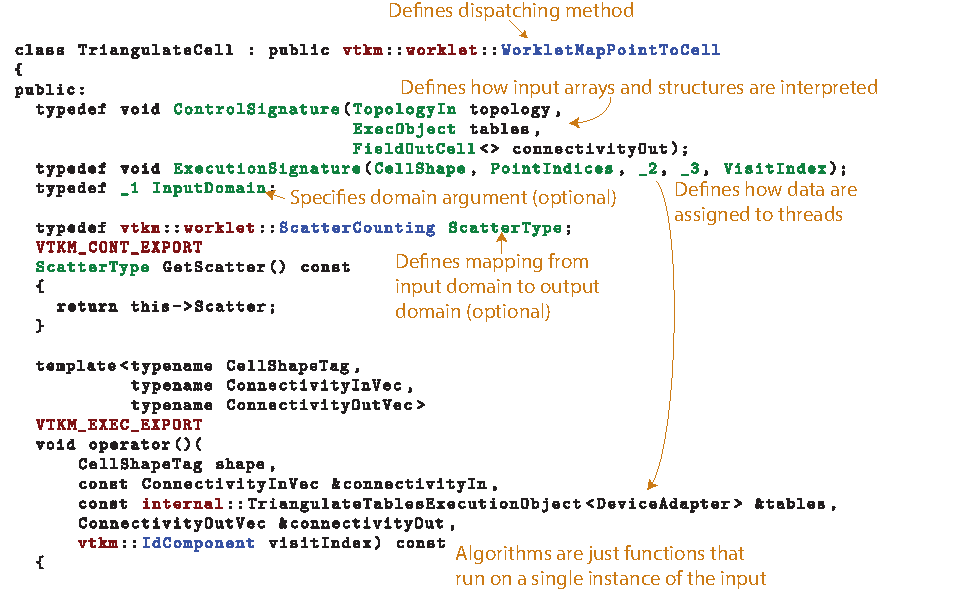
\includegraphics[width=\linewidth]{images/WorkletExampleAnnotated}
  \caption{Annotated example of a worklet declaration.}
  \label{fig:WorkletExampleAnnotated}
\end{figure}

\subsection{Control Signature}
\label{sec:ControlSignature}

\index{control~signature|(}
\index{signature!control|(}
\index{worklet!control~signature|(}

The control signature of a worklet is the \textcode{typedef} of a function
prototype named \controlsignature. The function prototype matches the
calling specification used with the dispatcher \textcode{Invoke} function.

\vtkmlisting{A \protect\controlsignature.}{ControlSignature.cxx}

The return type of the function prototype is always \textcode{void} because
the dispatcher \textcode{Invoke} functions do not return values. The
parameters of the function prototype are \index{signature tags}\keyterm{tags}
that identify the type of data that is expected to be passed to invoke.
\controlsignature tags are defined by the worklet type and the various tags
are documented more fully in Section~\ref{sec:CreatingWorkletsOfType}.

By convention, \controlsignature tag names start with the base concept
(e.g. \textsignature{Field} or \textsignature{Topology}) followed by the
domain (e.g. \textsignature{Point} or \textsignature{Cell}) followed by
\textsignature{In} or \textsignature{Out}. For example,
\sigtag{FieldPointIn} would specify values for a field on the points of a
mesh that are used as input (read only). Although they should be there in
most cases, some tag names might leave out the domain or in/out parts if
they are obvious or ambiguous.

\subsubsection{Type List Tags}
\label{sec:TypeListTags}

\index{type~list~tags|(}
\index{control~signature!type~list~tags|(}

Some tags are templated to have modifiers. For example,
\textsignature{Field} tags have a template argument that is set to a type
list tag defining what types of field data are supported. (See
Section~\ref{sec:TypeLists} for a description of type lists.) In fact, this
type list modifier is so common that the following convenience subtags used
with \textsignature{Field} tags are defined for all worklet types.

\begin{description}
  \label{TypeTagList}
\item[\sigtag{AllTypes}] All possible types.
\item[\sigtag{CommonTypes}] The most used types in visualization. This
  includes signed integers and floats that are 32 or 64 bit. It also
  includes 3 dimensional vectors of floats. The same as
  \vtkm{TypeListTagCommon}.
\item[\sigtag{IdType}] Contains the single item \vtkm{Id}. The same as
  \vtkm{TypeListTagId}.
\item[\sigtag{Id2Type}] Contains the single item \vtkm{Id2}. The same as
  \vtkm{TypeListTagId2}.
\item[\sigtag{Id3Type}] Contains the single item \vtkm{Id3}. The same as
  \vtkm{TypeListTagId3}.
\item[\sigtag{Index}] All types used to index arrays. Contains \vtkm{Id},
  \vtkm{Id2}, and \vtkm{Id3}. The same as \vtkm{TypeListTagIndex}.
\item[\sigtag{FieldCommon}] A list containing all the types generally
  used for fields. It is the combination of \sigtag{Scalar}, \sigtag{Vec2},
  \sigtag{Vec3}, and \sigtag{Vec4}. The same as \vtkm{TypeListTagField}.
\item[\sigtag{Scalar}] Types used for scalar fields. Specifically, it
  contains floating point numbers of different widths (i.e. \vtkm{Float32}
  and \vtkm{Float64}). The same as \vtkm{TypeListTagFieldScalar}.
\item[\sigtag{ScalarAll}] All scalar types. It contains signed and unsigned
  integers of widths from 8 to 64 bits. It also contains floats of 32 and
  64 bit widths. The same as \vtkm{TypeListTagScalarAll}.
\item[\sigtag{Vec2}] Types for values of fields with 2 dimensional
  vectors. All these vectors use floating point numbers. The same as
  \vtkm{TypeListTagFieldVec2}.
\item[\sigtag{Vec3}] Types for values of fields with 3 dimensional
  vectors. All these vectors use floating point numbers. The same as
  \vtkm{TypeListTagFieldVec3}.
\item[\sigtag{Vec4}] Types for values of fields with 4 dimensional
  vectors. All these vectors use floating point numbers. The same as
  \vtkm{TypeListTagFieldVec4}.
\item[\sigtag{VecAll}] All \vtkm{Vec} classes with standard integers or
  floating points as components and lengths between 2 and 4. The same as
  \vtkm{TypeListTagVecAll}.
\item[\sigtag{VecCommon}] The most common vector types. It contains all
  \vtkm{Vec} class of size 2 through 4 containing components of unsigned
  bytes, signed 32-bit integers, signed 64-bit integers, 32-bit floats, or
  64-bit floats. The same as \vtkm{TypeListTagVecCommon}.
\end{description}

\index{control~signature!type~list~tags|)}
\index{type~list~tags|)}

\index{worklet!control~signature|)}
\index{signature!control|)}
\index{control~signature|)}

\subsection{Execution Signature}
\label{sec:ExecutionSignature}

\index{execution~signature|(}
\index{signature!execution|(}
\index{worklet!execution~signature|(}

Like the control signature, the execution signature of a worklet is the
\textcode{typedef} of a function prototype named \executionsignature. The
function prototype must match the parenthesis operator (described in
Section~\ref{sec:WorkletOperator}) in terms of arity and argument
semantics.

\vtkmlisting{An \protect\executionsignature.}{ExecutionSignature.cxx}

The arguments of the \executionsignature's function prototype are tags that
define where the data come from. The most common tags are an underscore
followed by a number, such as \sigtagnum{1}, \sigtagnum{2}, etc. These
numbers refer back to the corresponding argument in the
\controlsignature. For example, \sigtagnum{1} means data from the first
control signature argument, \sigtagnum{2} means data from the second
control signature argument, etc.

Unlike the control signature, the execution signature optionally can
declare a return type if the parenthesis operator returns a value. If this
is the case, the return value should be one of the numeric tags
(i.e. \sigtagnum{1}, \sigtagnum{2}, etc.) to refer to one of the data
structures of the control signature. If the parenthesis operator does not
return a value, then \executionsignature should declare the return type as
\textcode{void}.

In addition to the numeric tags, there are other execution signature tags
to represent other types of data. For example, the \sigtag{WorkIndex} tag
identifies the instance of the worklet invocation. Each call to the worklet
function will have a unique \sigtag{WorkIndex}. Other such tags exist and
are described in the following section on worklet types where appropriate.

\index{worklet!execution~signature|)}
\index{signature!execution|)}
\index{execution~signature|)}

\subsection{Input Domain}
\label{sec:InputDomain}

\index{input domain|(}
\index{worklet!input~domain|(}

All worklets represent data parallel operations that are executed over
independent elements in some domain. The type of domain is inherent from
the worklet type, but the size of the domain is dependent on the data being
operated on. One of the arguments given to the dispatcher's
\textcode{Invoke} in the control environment must specify the domain.

A worklet identifies the argument specifying the domain with a
\textcode{typedef} named \inputdomain. The \inputdomain must be
\textcode{typedef}ed to one of the execution signature numeric tags
(i.e. \sigtagnum{1}, \sigtagnum{2}, etc.). By default, the \inputdomain
points to the first argument, but a worklet can override that to point to
any argument.

\vtkmlisting{An \protect\inputdomain declaration.}{InputDomain.cxx}

Different types of worklets can have different types of domain. For example
a simple field map worklet has a \sigtag{FieldIn} argument as its input
domain, and the size of the input domain is taken from the size of the
associated field array. Likewise, a worklet that maps topology has a
\sigtag{TopologyIn} argument as its input domain, and the size of the input
domain is taken from the cell set.

Specifying the \inputdomain is optional. If it is not specified, the first
argument is assumed to be the input domain.

\index{worklet!input~domain|)}
\index{input domain|)}

\subsection{Worklet Operator}
\label{sec:WorkletOperator}

A worklet is fundamentally a functor that operates on an element of data.
Thus, the algorithm that the worklet represents is contained in or called
from the parenthesis operator method.

\vtkmlisting{An overloaded parenthesis operator of a worklet.}{WorkletOperator.cxx}

There are some constraints on the parenthesis operator. First, it must have
the same arity as the \executionsignature, and the types of the parameters
and return must be compatible. Second, because it runs in the execution
environment, it must be declared with the \vtkmexecexport (or
\vtkmexeccontexport) modifier. Third, the method must be declared
\textcode{const} to help preserve thread safety.

\subsection{Worklet Types}
\label{sec:CreatingWorkletsOfType}

\index{worklet~types|(}

There are multiple worklet types provided by VTK-m, each designed to
support a particular type of operation. This section will define each of
the worklet types, identify the generic superclass that a worklet instance
should derive, identify the signature tags and their meanings, and give an
example of the worklet in use.

\newcommand{\commoncontrolsignaturetags}{
\item[\sigtag{WholeArrayIn}] This tag represents an array where all entries
  can be read by every worklet invocation. A \sigtag{WholeArrayIn} argument
  expects an \textidentifier{ArrayHandle} in the associated parameter of
  the dispatcher's \textcode{Invoke}. An array portal capable of reading
  from any place in the array is given to the worklet. Whole arrays are
  discussed in detail in Section~\ref{sec:WholeArrays} starting on
  page~\pageref{sec:WholeArrays}.

\item[\sigtag{WholeArrayOut}] This tag represents an array where any entry
  can be written by any worklet invocation. A \sigtag{WholeArrayOut}
  argument expects an \textidentifier{ArrayHandle} in the associated
  parameter of the dispatcher's \textcode{Invoke}. An array portal capable
  of writing to any place in the array is given to the worklet. Developers
  should take care when using writable whole arrays as introducing race
  conditions is possible. Whole arrays are discussed in detail in
  Section~\ref{sec:WholeArrays} starting on page~\pageref{sec:WholeArrays}.

\item[\sigtag{WholeArrayInOut}] This tag represents an array where any
  entry can be read or written by any worklet invocation. A
  \sigtag{WholeArrayInOut} argument expects an \textidentifier{ArrayHandle}
  in the associated parameter of the dispatcher's \textcode{Invoke}. An
  array portal capable of reading from or writing to any place in the array
  is given to the worklet. Developers should take care when using writable
  whole arrays as introducing race conditions is possible. Whole arrays are
  discussed in detail in Section~\ref{sec:WholeArrays} starting on
  page~\pageref{sec:WholeArrays}.

\item[\sigtag{ExecObject}] This tag represents an execution object that is
  passed directly from the control environment to the worklet. A
  \sigtag{ExecObject} argument expects a subclass of
  \vtkmexec{ExecutionObjectBase}, and this same object is given to the
  worklet. Execution objects are discussed in detail in
  Section~\ref{sec:ExecutionObjects} starting on
  page~\pageref{sec:ExecutionObjects}.
}

\newcommand{\numericexecutionsignaturetags}{
\item[\sigtagnum{1}, \sigtagnum{2},$\ldots$] These reference the
  corresponding parameter in the \controlsignature.
}

\newcommand{\commonexecutionsignaturetags}{
\item[\sigtag{WorkIndex}] This tag produces a \vtkm{Id} that uniquely
  identifies the invocation of the worklet.
\item[\sigtag{VisitIndex}] This tag produces a \vtkm{IdComponent} that
  uniquely identifies when multiple worklet invocations operate on the same
  input item, which can happen when defining a worklet with scatter (as
  described in Section~\ref{sec:WorkletScatter}).
}

\subsubsection{Field Map}

\index{worklet~types!field~map|(}
\index{field~map~worklet|(}
\index{map~field|(}

A worklet deriving \vtkmworklet{WorkletMapField} performs a basic mapping
operation that applies a function (the operator in the worklet) on all the
field values at a single point or cell and creates a new field value at
that same location. Although the intention is to operate on some variable
over the mesh, a \textidentifier{WorkletMapField} can actually be applied
to any array.

A \textidentifier{WorkletMapField} subclass is invoked with a
\vtkmworklet{DispatcherMapField}. This dispatcher has two template
arguments. The first argument is the type of the worklet subclass. The
second argument, which is optional, is a device adapter tag.

A field map worklet supports the following tags in the parameters of its
\controlsignature.

\begin{description}
\item[\sigtag{FieldIn}] This tag represents an input field. A
  \sigtag{FieldIn} argument expects an \textidentifier{ArrayHandle} or a
  \textidentifier{DynamicArrayHandle} in the associated parameter of the
  dispatcher's \textcode{Invoke}. Each invocation of the worklet gets a
  single value out of this array.

  \sigtag{FieldIn} has a single template parameter that specifies what data
  types are acceptable for the array. The type tags are described in
  Section~\ref{sec:TypeListTags} starting on
  page~\pageref{TypeTagList}.

  The worklet's \inputdomain can be set to a \sigtag{FieldIn} argument. In
  this case, the input domain will be the size of the array.

\item[\sigtag{FieldOut}] This tag represents an output field. A
  \sigtag{FieldOut} argument expects an \textidentifier{ArrayHandle} or a
  \textidentifier{DynamicArrayHandle} in the associated parameter of the
  dispatcher's \textcode{Invoke}. The array is resized before scheduling
  begins, and each invocation of the worklet sets a single value in the
  array.

  \sigtag{FieldOut} has a single template parameter that specifies what
  data types are acceptable for the array. The type tags are described in
  Section~\ref{sec:TypeListTags} starting on
  page~\pageref{TypeTagList}.

\item[\sigtag{FieldInOut}] This tag represents field that is both an input
  and an output. A \sigtag{FieldInOut} argument expects an
  \textidentifier{ArrayHandle} or a \textidentifier{DynamicArrayHandle} in
  the associated parameter of the dispatcher's \textcode{Invoke}. Each
  invocation of the worklet gets a single value out of this array, which is
  replaced by the resulting value after the worklet completes.

  \sigtag{FieldInOut} has a single template parameter that specifies what
  data types are acceptable for the array. The type tags are described in
  Section~\ref{sec:TypeListTags} starting on
  page~\pageref{TypeTagList}.

  The worklet's \inputdomain can be set to a \sigtag{FieldInOut} argument. In
  this case, the input domain will be the size of the array.

  \commoncontrolsignaturetags
\end{description}

A field map worklet supports the following tags in the parameters of its
\executionsignature.

\begin{description}
  \numericexecutionsignaturetags

  \commonexecutionsignaturetags
\end{description}

Field maps most commonly perform basic calculator arithmetic, as
demonstrated in the following example.

\vtkmlisting{Declaration and use of a field map worklet.}{UseWorkletMapField.cxx}

Although simple, the \textidentifier{WorkletMapField} worklet type can be
used (and abused) as a general parallel-for/scheduling mechanism. In
particular, the \sigtag{WorkIndex} execution signature tag can be used to
get a unique index, the \textsignature{WholeArray}* tags can be used to get
random access to arrays, and the \sigtag{ExecObject} control signature tag
can be used to pass execution objects directly to the worklet.

\fix{This discussion needs to be updated to use \sigtag{WholeArrayOut}. It
  also needs to reference sections \ref{sec:WholeArrays} and
  \ref{sec:ExecutionObjects}.}

The \sigtag{ExecObject} parameter can be used in conjunction with the
\vtkmexec{ExecutionWholeArray} class to pass an entire array into a
worklet. \textidentifier{ExecutionWholeArray} takes an
\textidentifier{ArrayHandle} object in the control environment and converts
it to an execution environment object that is compatible with the
\sigtag{ExecObject} tag. This allows you to have random access to the
array. (You can also use \vtkmexec{ExecutionWholeArrayConst} for read only
access.) Care should be taken when directly accessing an array like this.
Be sure to avoid invalid indexing or memory race conditions, which can be
hard to debug.

The following example uses the random access of
\textidentifier{ExecutionWholeArray} to make a worklet that copies an array
in reverse order.

\vtkmlisting{Using \textidentifier{ExecutionWholeArray} for random array access.}{RandomArrayAccess.cxx}

\index{map~field|)}
\index{field~map~worklet|)}
\index{worklet~types!field~map|)}

\subsubsection{Topology Map}
\label{sec:WorkletMapTopology}

\index{worklet~types!topology~map|(}
\index{topology~map~worklet|(}
\index{map~topology|(}

\index{map~topology|)}
\index{topology~map~worklet|)}
\index{worklet~types!topology~map|)}

\subsubsection{Point to Cell Map}
\label{sec:WorkletMapPointToCell}

\index{worklet~types!point~to~cell~map|(}
\index{point~to~cell~map~worklet|(}
\index{map~point~to~cell|(}

\index{map~point~to~cell|)}
\index{point~to~cell~map~worklet|)}
\index{worklet~types!point~to~cell~map|)}

\fix{When is cell to point map going to be implemented?}

%% \subsubsection{Cell to Point Map}
%% \label{sec:WorkletMapCellToPoint}

%% \index{worklet~types!cell~to~point~map|(}
%% \index{cell~to~point~map~worklet|(}
%% \index{map~cell~to~point|(}

%% \index{map~cell~to~point|)}
%% \index{cell~to~point~map~worklet|)}
%% \index{worklet~types!cell~to~point~map|)}


%% \subsubsection{Cell Map}

%% \index{worklet~types!cell~map|(}
%% \index{cell~map~worklet|(}
%% \index{map~cell|see{cell map worklet}}

%% A worklet deriving \daxexec{WorkletMapCell} performs a mapping operation
%% that applies a function (the operator in the worklet) on field values on a
%% single cell and creates a new field value at that location. The function
%% has access to all field values local to that cell. So if an input is a
%% point field, the operation will have access to all the values of that
%% field.

%% A \textidentifier{WorkletMapCell} subclass is invoked with a
%% \daxcont{DispatcherMapCell}. This dispatcher has two template
%% arguments. The first argument is the type of the worklet subclass. The
%% second argument, which is optional, is a device adapter tag.

%% A cell map worklet supports the following tags in the parameters of its
%% \controlsignature.
%% \begin{description}
%% \item[\sigtag{Topology}] This tag corresponds to one of the grid structures
%%   described in Section~\ref{sec:GridStructures} passed to invoke that holds
%%   the topology on which to apply the map.

%%   If the \sigtag{Topology} argument is referenced with a numeric tag in the
%%   \executionsignature (e.g. with \sigtagnum{1}), then the worklet operator
%%   receives the cell-type tag (such as \dax{CellTagTriangle} or
%%   \dax{CellTagVoxel}). This is sometimes useful for specializing   based
%%   on the cell type, but usually unnecessary.

%%   If the \sigtag{Topology} argument is referenced by a \sigtag{Vertices}
%%   tag wrapping a numeric tag (e.g. with \sigtagmodnum{Vertices}{1}), then
%%   the worklet function is passed a \daxexec{CellVertices} object that
%%   contains the point indices for all the vertices of the cell.
%% \item[\sigtag{Field}] This tag corresponds to a \daxcont{ArrayHandle}
%%   passed to invoke that holds the sample values for a field at all points
%%   or all cells. The \sigtag{Field} tag can be modified to be either
%%   \sigtag{In} (the default) or \sigtag{Out}. Input \sigtag{Field} tags can
%%   be further modified to be attached to \sigtag{Point}s or
%%   \sigtag{Cell}s. The size of the input \daxcont{ArrayHandle} must match
%%   the number of points or cells in the grid structure passed in as a
%%   \sigtag{Topology} argument.  Output fields are always attached to the
%%   cells, and the corresponding \daxcont{ArrayHandle} will be resized as
%%   necessary.

%%   A cell field has a one-to-one mapping between \daxcont{ArrayHandle}
%%   entries and worklet function parameters. Thus, when the
%%   \executionsignature references a \controlsignature \sigtag{Field}
%%   parameter (e.g. with \sigtagnum{2}), the parameter is the same as the
%%   basic type as the values in the array (typically something like
%%   \dax{Scalar} or \dax{Vector3}).

%%   A point field has a many-to-one mapping between \daxcont{ArrayHandle}
%%   entries and worklet function parameters because each cell can touch
%%   multiple points. So when a \daxcont{ArrayHandle} is translated to the
%%   worklet invocation, its values get passed in a \daxexec{CellField}
%%   object, which behaves like a \dax{Tuple} with a size matching the number
%%   of vertices in a cell.
%% \end{description}

%% A cell map worklet supports the following tags in the parameters of its
%% \executionsignature.
%% \begin{description}
%% \item[\sigtagnum{1}, \sigtagnum{2},$\ldots$] These reference the
%%   corresponding parameter in the \controlsignature.
%% \item[\sigtag{Vertices}] When modified by one of the numeric tags
%%   (e.g. \sigtagmodnum{Vertices}{1}), passes a \daxexec{CellVertices} to the
%%   worklet representing the point indices for each vertex of the cell.
%% \item[\sigtag{WorkId}] Produces a \dax{Id} that uniquely identifies the
%%   invocation instance of the worklet.
%% \end{description}

%% Cell maps most commonly perform operations on interpolated fields. They
%% often use the cell operations provided by the Dax toolkit and described in
%% Section~\ref{sec:CellsAndOperations}. The following example shows a cell
%% map worklet that simply averages all the point values it touches. A more
%% serious worklet would probably perform interpolations, derivatives, or
%% integrations over the cell.

%% \begin{daxexample}{Declaration and use of a cell map worklet.}
%% #include <dax/exec/WorkletMapCell.h>

%% #include <dax/exec/CellField.h>

%% #include <dax/cont/ArrayHandle.h>
%% #include <dax/cont/DispatcherMapCell.h>
%% #include <dax/cont/UniformGrid.h>

%% class CellAverage : public dax::exec::WorkletMapCell
%% {
%% public:
%%   typedef void ControlSignature(Topology, Field(Point), Field(Out));
%%   typedef _3 ExecutionSignature(_1,_2);

%%   template<class CellTag>
%%   DAX_EXEC_EXPORT
%%   dax::Scalar operator()(
%%     CellTag, const dax::exec::CellField<dax::Scalar,CellTag> &values) const
%%   {
%%     dax::Scalar sum = values[0];
%%     for (int index = 1; index < values.NUM_VERTICES; index++)
%%       {
%%       sum += values[index];
%%       }
%%     return sum/values.NUM_VERTICES;
%%   }
%% };

%% DAX_CONT_EXPORT
%% void InvokeCellAverage()
%% {
%%   const dax::Id DIM = 100;

%%   // Make a grid structure.
%%   dax::cont::UniformGrid<> grid;
%%   grid.SetExtent(dax::make_Id3(0, 0, 0), dax::make_Id3(DIM-1, DIM-1, DIM-1));

%%   // Make input.
%%   // (A real application would make more interesting data and do it more efficiently.)
%%   dax::Scalar inputBuffer[DIM*DIM*DIM];
%%   for (dax::Id index = 0; index < DIM*DIM*DIM; index++)
%%     {
%%     inputBuffer[index] = index;
%%     }
%%   dax::cont::ArrayHandle<dax::Scalar> input =
%%       dax::cont::make_ArrayHandle(inputBuffer, DIM*DIM*DIM);

%%   dax::cont::ArrayHandle<dax::Scalar> output;

%%   dax::cont::DispatcherMapCell<CellAverage> dispatcher;
%%   dispatcher.Invoke(grid, input, output);

%%   // Do something with output.
%% }

%% \end{daxexample}

%% \index{cell~map~worklet|)}
%% \index{worklet~types!cell map|)}

%% \subsubsection{Generate Topology}

%% \index{worklet~types!generate~topology|(}
%% \index{generate~topology~worklet|(}

%% A worklet deriving from \daxexec{WorkletGenerateTopology} generates a cell
%% connectivity. When invoked, the dispatcher is given an array containing the
%% number of output cells derived from each input cell. Each invocation of a
%% \daxexec{WorkletGenerateTopology} produces exactly one cell, so the
%% dispatcher then invokes the generate topology worklet multiple times per
%% cell if multiple cells are derived.

%% A \textidentifier{WorkletGenerateTopology} subclass is invoked with a
%% \daxcont{DispatcherGenerateTopology}. This dispatcher has three template
%% arguments. The first argument is the type of the worklet subclass. The
%% second argument is a type of array handle (defaults to
%% \daxcont{ArrayHandle}\textcode{<}\dax{Id}\textcode{>}) that holds the count
%% of cells to be generated per input value. The third argument, which is
%% optional, is a device adapter tag.

%% Generate topology operations are used when one topology is derived from
%% another's points. A generate topology is often proceeded by a field map or
%% cell map that counts how many cells will be derived from each input
%% cell. These counts are stored in an array and passed to the
%% \daxcont{DispatcherGenerateTopology} that invokes the worklet.

%% A generate topology worklet supports the following tags in the parameters
%% of its \controlsignature.
%% \begin{description}
%% \item[\sigtag{Topology}] This tag corresponds to one of the grid structures
%%   described in Section~\ref{sec:GridStructures} passed to invoke that holds
%%   the topology on which to derive a new topology or to write the new
%%   topology into. The \sigtag{Topology} tag can be modified to be either
%%   \sigtag{In} (the default) or \sigtag{Out}.

%%   If the \sigtag{Topology} argument is referenced with a numeric tag in the
%%   \executionsignature (e.g. with \sigtagnum{1}), then the worklet operator
%%   receives the cell-type tag (such as \dax{CellTagTriangle} or
%%   \dax{CellTagVoxel}). This is sometimes useful for specializing   based
%%   on the cell type, but usually unnecessary.

%%   If the \sigtag{Topology} argument is referenced by a \sigtag{Vertices}
%%   tag wrapping a numeric tag (e.g. with \sigtagmodnum{Vertices}{1}), then
%%   the worklet function is passed a \daxexec{CellVertices} object that
%%   contains the point indices for all the vertices of the cell.
%% \item[\sigtag{Field}] This tag corresponds to a \daxcont{ArrayHandle}
%%   passed to invoke that holds the sample values for a field at all points
%%   or all cells. All fields for generate topology worklets are input. The
%%   \sigtag{Field} tag can be modified to be attached to \sigtag{Point}s or
%%   \sigtag{Cell}s. The size of the \daxcont{ArrayHandle} must match the
%%   number of points or cells in the grid structure passed in as a
%%   \sigtag{Topology} argument.

%%   A cell field has a one-to-one mapping between \daxcont{ArrayHandle}
%%   entries and worklet function parameters. Thus, when the
%%   \executionsignature references a \controlsignature \sigtag{Field}
%%   parameter (e.g. with \sigtagnum{2}), the parameter is the same as the
%%   basic type as the values in the array (typically something like
%%   \dax{Scalar} or \dax{Vector3}).

%%   A point field has a many-to-one mapping between \daxcont{ArrayHandle}
%%   entries and worklet function parameters because each cell can touch
%%   multiple points. So when a \daxcont{ArrayHandle} is translated to the
%%   worklet invocation, its values get passed in a \daxexec{CellField}
%%   object, which behaves like a \dax{Tuple} with a size matching the number
%%   of vertices in a cell.
%% \end{description}

%% A generate topology worklet supports the following tags in the parameters
%% of its \executionsignature.
%% \begin{description}
%% \item[\sigtagnum{1}, \sigtagnum{2},$\ldots$] These reference the
%%   corresponding parameter in the \controlsignature.
%% \item[\sigtag{Vertices}] When modified by one of the numeric tags
%%   (e.g. \sigtagmodnum{Vertices}{1}), passes a \daxexec{CellVertices} to the
%%   worklet representing the point indices for each vertex of the cell. The
%%   numeric tag must point to a \controlsignature parameter of type
%%   \sigtag{Topology}.
%% \item[\sigtag{VisitId}] Produces a \dax{Id} that uniquely identifies the
%%   invocation instance for the particular cell being visited. For example,
%%   if dividing hexahedra into tetrahedra, each hexahedra produces 5 or 6
%%   tetrahedra, but each invocation of the generate topology worklet
%%   generates just one of this. The \sigtag{VisitId} identifies which of the
%%   tetrahedra to produce.
%% \item[\sigtag{WorkId}] Produces a \dax{Id} that uniquely identifies the
%%   invocation instance of the worklet.
%% \end{description}

%% The following example converts a uniform grid of voxels into the a
%% collection of quadrilaterals that make up the faces. The worklet leverages
%% the implicit topology of a uniform grid to ensure that each face is
%% represented exactly once.

%% \begin{daxexample}{Declaration and use of a generate topology worklet.}
%% #include <dax/exec/WorkletGenerateTopology.h>

%% #include <dax/Extent.h>

%% #include <dax/exec/CellVertices.h>
%% #include <dax/exec/WorkletMapCell.h>

%% #include <dax/cont/ArrayHandle.h>
%% #include <dax/cont/DispatcherGenerateTopology.h>
%% #include <dax/cont/DispatcherMapCell.h>
%% #include <dax/cont/UniformGrid.h>
%% #include <dax/cont/UnstructuredGrid.h>

%% DAX_EXEC_CONSTANT_EXPORT
%% const unsigned char VoxelFaces[6][4] = {
%%   { 0, 3, 7, 4 },
%%   { 0, 4, 5, 1 },
%%   { 0, 1, 2, 3 },
%%   { 1, 2, 6, 5 },
%%   { 2, 3, 7, 6 },
%%   { 4, 5, 6, 7 }
%% };

%% class CountFaceOut : public dax::exec::WorkletMapCell
%% {
%% public:
%%   typedef void ControlSignature(Topology, Field(Out), Field(Out));
%%   typedef _3 ExecutionSignature(WorkId, _2);

%%   DAX_CONT_EXPORT
%%   CountFaceOut(dax::Id3 dimensions) : Dimensions(dimensions) {  }

%%   DAX_EXEC_EXPORT
%%   dax::Id operator()(dax::Id workId, dax::Tuple<unsigned char,6> &faceToOutput) const
%%   {
%%     dax::Id3 index3D;
%%     dax::Id flatIndex = workId;
%%     for (i = 0; i < 3; i++)
%%       {
%%       index3D[i] = flatIndex % this->Dimensions[i];
%%       flatIndex /= this->Dimensions[i];
%%       }

%%     dax::Id count = 0;
%%     // First three faces output on all cells.
%%     faceToOutput[count] = 0;  count++;
%%     faceToOutput[count] = 1;  count++;
%%     faceToOutput[count] = 2;  count++;

%%     // Second three faces output only on cells at maximum boundary.
%%     if (flatIndex[0] == this->Dimensions[0]-1) { faceToOutput[count] = 3;  count++; }
%%     if (flatIndex[1] == this->Dimensions[1]-1) { faceToOutput[count] = 4;  count++; }
%%     if (flatIndex[2] == this->Dimensions[2]-1) { faceToOutput[count] = 5;  count++; }

%%     return count;
%%   }

%% private:
%%   dax::Id3 Dimensions;
%% };

%% class ExtractFace : public dax::exec::WorkletGenerateTopology
%% {
%% public:
%%   typedef void ControlSignature(Topology, Topology(Out), Field);
%%   typedef void ExecutionSignature(Vertices(_1), Vertices(_2), _3, VisitIndex);

%%   DAX_EXEC_EXPORT
%%   void operator()(const dax::exec::CellVertices<dax::CellTagVoxel> &inVertices,
%%                   dax::exec::CellVertices<dax::CellTagQuadrilateral> &outVertices,
%%                   const dax::Tuple<unsigned char,6> outputFaces,
%%                   dax::Id visitIndex) const
%%   {
%%     unsigned char faceId = outputFaces[visitIndex];
%%     outVertices[0] = inVertices[VoxelFaces[faceId][0]];
%%     outVertices[1] = inVertices[VoxelFaces[faceId][1]];
%%     outVertices[2] = inVertices[VoxelFaces[faceId][2]];
%%     outVertices[3] = inVertices[VoxelFaces[faceId][3]];
%%   }
%% };

%% DAX_CONT_EXPORT
%% dax::cont::UnstructuredGrid<dax::CellTagQuadrilateral>
%% InvokeExtraceFaces(const dax::cont::UniformGrid<> &inputGrid)
%% {
%%   dax::Id3 dimensions = dax::extentCellDimensions(inputGrid.GetExtent());

%%   dax::cont::ArrayHandle<dax::Tuple<unsigned char,6> > faces;
%%   dax::cont::ArrayHandle<dax::Id> counts;

%%   dax::cont::DispatcherMapCell<CountFaceOut> countDispatcher(CountFaceOut(dimensions));
%%   countDispatcher.Invoke(inputGrid, faces, counts);

%%   dax::cont::UnstructuredGrid<dax::CellTagQuadrilateral> outputGrid;

%%   dax::cont::DispatcherGenerateTopology<ExtractFace> extractFaceDispatcher(counts);
%%   extractFaceDispatcher.SetRemoveDuplicatePoints(false); // All points will be used.
%%   extractFaceDispatcher.Invoke(inputGrid, outputGrid, faces);

%%   return outputGrid;
%% }
%% \end{daxexample}

%% \index{generate~topology~worklet|)}
%% \index{worklet~types!generate~topology|)}

%% \subsubsection{Interpolated Cell}

%% \index{worklet~types!interpolated~cell|(}
%% \index{interpolated~cell~worklet|(}

%% A worklet deriving from \daxexec{WorkletInterpolatedCell} generates a new
%% geometry comprising both new points at new coordinates and cell connections
%% among those points. When invoked, the dispatcher is given an array
%% containing the number of cells produced. (The cell type must be
%% homogeneous.) Each invocation of a \daxexec{WorkletInterpolatedCell}
%% produces exactly one cell and its associated points, so the dispatcher then
%% invokes the interpolated cell worklet multiple times per cell if multiple
%% cells are derived.

%% A \textidentifier{WorkletInterpolatedCell} subclass is invoked with a
%% \daxcont{DispatcherInterpolatedCell}. This dispatcher has three template
%% arguments. The first argument is the type of the worklet subclass. The
%% second argument is a type of array handle (defaults to
%% \daxcont{ArrayHandle}\textcode{<}\dax{Id}\textcode{>}) that holds the count
%% of cells to be generated per input value. The third argument, which is
%% optional, is a device adapter tag.

%% Interpolated cell operations are used when one topology is derived from
%% another, but the new topology can build cells in unconstrained ways. An
%% interpolated cell is often proceeded by a field map or cell map that counts
%% how many cells will be derived from each input cell. These counts are
%% stored in an array and passed to the \daxcont{DispatcherInterpolatedCell}
%% that invokes the worklet.

%% An interpolated cell worklet supports the following tags in the parameters
%% of its \controlsignature.
%% \begin{description}
%% \item[\sigtag{Topology}] This tag corresponds to one of the grid structures
%%   described in Section~\ref{sec:GridStructures} passed to invoke that holds
%%   the topology on which to derive a new topology.

%%   If the \sigtag{Topology} argument is referenced with a numeric tag in the
%%   \executionsignature (e.g. with \sigtagnum{1}), then the worklet operator
%%   receives the cell-type tag (such as \dax{CellTagTriangle} or
%%   \dax{CellTagVoxel}). This is sometimes useful for specializing   based
%%   on the cell type, but usually unnecessary.

%%   If the \sigtag{Topology} argument is referenced by a \sigtag{Vertices}
%%   tag wrapping a numeric tag (e.g. with \sigtagmodnum{Vertices}{1}), then
%%   the worklet function is passed a \daxexec{CellVertices} object that
%%   contains the point indices for all the vertices of the cell.
%% \item[\sigtag{Geometry}] This tag corresponds to one of the grid structures
%%   described in Section~\ref{sec:GridStructures} passed to
%%   invoke. Parameters of this type access the full geometry of the grid
%%   including both point locations and cell connections. The
%%   \sigtag{Geometry} tag is always used in the output of an interpolated
%%   cell worklet, and so should be modified with \sigtag{Out}.

%%   When the \executionsignature references a \controlsignature
%%   \sigtag{Geometry} parameter (e.g. with \sigtagnum{2}), the parameter is a
%%   \daxexec{InterpolatedCellPoints} object. The worklet operator should pass
%%   this parameter by reference so that it may be filled and the results
%%   returned.
%% \item[\sigtag{Field}] This tag corresponds to a \daxcont{ArrayHandle}
%%   passed to invoke that holds the sample values for a field at all points
%%   or all cells. All fields for generate topology worklets are input. The
%%   \sigtag{Field} tag can be modified to be attached to \sigtag{Point}s or
%%   \sigtag{Cell}s. The size of the \daxcont{ArrayHandle} must match the
%%   number of points or cells in the grid structure passed in as a
%%   \sigtag{Topology} argument.

%%   A cell field has a one-to-one mapping between \daxcont{ArrayHandle}
%%   entries and worklet function parameters. Thus, when the
%%   \executionsignature references a \controlsignature \sigtag{Field}
%%   parameter (e.g. with \sigtagnum{2}), the parameter is the same as the
%%   basic type as the values in the array (typically something like
%%   \dax{Scalar} or \dax{Vector3}).

%%   A point field has a many-to-one mapping between \daxcont{ArrayHandle}
%%   entries and worklet function parameters because each cell can touch
%%   multiple points. So when a \daxcont{ArrayHandle} is translated to the
%%   worklet invocation, its values get passed in a \daxexec{CellField}
%%   object, which behaves like a \dax{Tuple} with a size matching the number
%%   of vertices in a cell.
%% \end{description}

%% An interpolated cell worklet supports the following tags in the parameters
%% of its \executionsignature.
%% \begin{description}
%% \item[\sigtagnum{1}, \sigtagnum{2},$\ldots$] These reference the
%%   corresponding parameter in the \controlsignature.
%% \item[\sigtag{Vertices}] When modified by one of the numeric tags
%%   (e.g. \sigtagmodnum{Vertices}{1}), passes a \daxexec{CellVertices} to the
%%   worklet representing the point indices for each vertex of the cell. The
%%   numeric tag must point to a \controlsignature parameter of type
%%   \sigtag{Topology}.
%% \item[\sigtag{VisitId}] Produces a \dax{Id} that uniquely identifies the
%%   invocation instance for the particular cell being visited. For example,
%%   if dividing hexahedra into tetrahedra, each hexahedra produces 5 or 6
%%   tetrahedra, but each invocation of the generate topology worklet
%%   generates just one of this. The \sigtag{VisitId} identifies which of the
%%   tetrahedra to produce.
%% \item[\sigtag{WorkId}] Produces a \dax{Id} that uniquely identifies the
%%   invocation instance of the worklet.
%% \end{description}

%% The following example performs a slice on a uniform grid using a plane that
%% is aligned with the x axis (parallel with the y-z plane). With these
%% constraints, we know that the intersection of every cell will be a
%% quadrilateral.

%% \begin{daxexample}{Declaration and use of an interpolated cell worklet.}
%% #include <dax/exec/WorkletInterpolatedCell.h>

%% #include <dax/exec/CellField.h>
%% #include <dax/exec/CellVertices.h>
%% #include <dax/exec/InterpolatedCellPoints.h>
%% #include <dax/exec/WorkletMapCell.h>

%% #include <dax/cont/ArrayHandle.h>
%% #include <dax/cont/DispatcherInterpolatedCell.h>
%% #include <dax/cont/DispatcherMapCell.h>
%% #include <dax/cont/UniformGrid.h>
%% #include <dax/cont/UnstructuredGrid.h>

%% class CountXSliceOut : public dax::exec::WorkletMapCell
%% {
%% public:
%%   typedef void ControlSignature(Topology, Field(Point), Field(Out));
%%   typedef _3 ExecutionSignature(_2);

%%   DAX_CONT_EXPORT
%%   CountXSliceOut(dax::Scalar xIntercept) : XIntercept(xIntercept) {  }

%%   DAX_EXEC_EXPORT
%%   dax::Id operator()(
%%       const dax::exec::CellField<dax::Vector3, dax::CellTagVoxel> &pointCoordinates) const
%%   {
%%     dax::Scalar minX = pointCoordinates[0][0];
%%     dax::Scalar maxX = pointCoordinates[6][0];

%%     return ((minX <= this->XIntercept) && (this->XIntercept < maxX)) ? 1 : 0;
%%   }

%% private:
%%   dax::Scalar XIntercept;
%% };

%% class XSlice : public dax::exec::WorkletInterpolatedCell
%% {
%% public:
%%   typedef void ControlSignature(Topology, Geometry(Out), Field(Point));
%%   typedef void ExecutionSignature(Vertices(_1), _2, _3);

%%   DAX_CONT_EXPORT
%%   XSlice(dax::Scalar xIntercept) : XIntercept(xIntercept) {  }

%%   DAX_EXEC_EXPORT
%%   void operator()(
%%       const dax::exec::CellVertices<dax::CellTagVoxel> &inVertices,
%%       dax::exec::InterpolatedCellPoints<dax::CellTagQuadrilateral> &outVertices,
%%       const dax::exec::CellField<dax::Vector3, dax::CellTagVoxel> &pointCoordinates) const
%%   {
%%     dax::Scalar minX = pointCoordinates[0][0];
%%     dax::Scalar maxX = pointCoordinates[6][0];
%%     dax::Scalar interpolant = (this->XIntercept - minX)/(maxX - minX);

%%     outVertices.SetInterpolationPoint(0, inVertices[0], inVertices[1], interpolant);
%%     outVertices.SetInterpolationPoint(1, inVertices[3], inVertices[2], interpolant);
%%     outVertices.SetInterpolationPoint(2, inVertices[4], inVertices[5], interpolant);
%%     outVertices.SetInterpolationPoint(3, inVertices[7], inVertices[6], interpolant);
%%   }

%% private:
%%   dax::Scalar XIntercept;
%% };

%% DAX_CONT_EXPORT
%% dax::cont::UnstructuredGrid<dax::CellTagQuadrilateral>
%% InvokeXSlice(const dax::cont::UniformGrid<> &inputGrid, dax::Scalar xIntercept)
%% {
%%   dax::cont::ArrayHandle<dax::Id> counts;

%%   dax::cont::DispatcherMapCell<CountXSliceOut> countDispatcher(CountXSliceOut(xIntercept));
%%   countDispatcher.Invoke(inputGrid, inputGrid.GetPointCoordinates(), counts);

%%   dax::cont::UnstructuredGrid<dax::CellTagQuadrilateral> outputGrid;

%%   dax::cont::DispatcherInterpolatedCell<XSlice> sliceDispatcher(count, XSlice(xIntercept));
%%   sliceDispatcher.SetRemoveDuplicatePoints(true);
%%   sliceDispatcher.Invoke(inputGrid, outputGrid, inputGrid.GetPointCoordinates());

%%   return outputGrid;
%% }
%% \end{daxexample}

%% \index{interpolated~cell~worklet|)}
%% \index{worklet~types!interpolated~cell|)}

%% \subsubsection{Generate Keys and Values}

%% \index{worklet~types!generate~keys~and~values|(}
%% \index{generate~keys~and~values~worklet|(}

%% A worklet deriving from \daxexec{WorkletGenerateKeysValues}, which is
%% designed to be used in conjunction with the reduce keys and values worklet,
%% is an experimental type of worklet that can be applied to a variety of
%% visualization algorithms. They allow an algorithm with a lot of
%% interdependence to operate with lots of concurrency by storing and
%% deferring the interdependent operation.

%% In operation the generate keys and values worklet works very much like a
%% cell map worklet except that it is able to produce a variable amount of
%% field values per cell. Each invocation of a
%% \daxexec{WorkletGenerateKeysValues} generates one set of keys and values,
%% so the dispatcher then invokes the worklet multiple times per cell if
%% multiple key-value sets are needed.

%% A \textidentifier{WorkletGenerateKeysValues} subclass is invoked with a
%% \daxcont{DispatcherGenerateKeysValues}. This dispatcher has three template
%% arguments. The first argument is the type of the worklet subclass. The
%% second argument is a type of array handle (defaults to
%% \daxcont{ArrayHandle}\textcode{<}\dax{Id}\textcode{>}) that holds the count
%% of cells to be generated per input value. The third argument, which is
%% optional, is a device adapter tag.

%% When invoking, the dispatcher needs to know how many key-values to produce
%% per cell. These counts are stored in an array and passed to the
%% \daxcont{DispatcherGenerateKeysValues} that invokes the worklet. If all
%% cells produced the same number of key-values, then the implicit
%% \daxcont{ArrayHandleConstant} can be used.

%% Although the \daxexec{WorkletGenerateKeysValues} worklet is expected to
%% generate keys and values which have distinct semantics, the worklet itself
%% does not distinguish between them. Instead, both keys and values are simply
%% considered output fields.

%% A generate keys and values worklet supports the following tags in the
%% parameters of its \controlsignature.
%% \begin{description}
%% \item[\sigtag{Topology}] This tag corresponds to one of the grid structures
%%   described in Section~\ref{sec:GridStructures} passed to invoke that holds
%%   the topology on which to apply the map.

%%   If the \sigtag{Topology} argument is referenced with a numeric tag in the
%%   \executionsignature (e.g. with \sigtagnum{1}), then the worklet operator
%%   receives the cell-type tag (such as \dax{CellTagTriangle} or
%%   \dax{CellTagVoxel}). This is sometimes useful for specializing   based
%%   on the cell type, but usually unnecessary.

%%   If the \sigtag{Topology} argument is referenced by a \sigtag{Vertices}
%%   tag wrapping a numeric tag (e.g. with \sigtagmodnum{Vertices}{1}), then
%%   the worklet function is passed a \daxexec{CellVertices} object that
%%   contains the point indices for all the vertices of the cell.
%% \item[\sigtag{Field}] This tag corresponds to a \daxcont{ArrayHandle}
%%   passed to invoke that holds the sample values for a field at all points
%%   or all cells. The \sigtag{Field} tag can be modified to be either
%%   \sigtag{In} (the default) or \sigtag{Out}. Input \sigtag{Field} tags can
%%   be further modified to be attached to \sigtag{Point}s or
%%   \sigtag{Cell}s. The size of the input \daxcont{ArrayHandle} must match
%%   the number of points or cells in the grid structure passed in as a
%%   \sigtag{Topology} argument.  Output fields are always attached to the
%%   cells, and the corresponding \daxcont{ArrayHandle} will be resized as
%%   necessary.

%%   A cell field has a one-to-one mapping between \daxcont{ArrayHandle}
%%   entries and worklet function parameters. Thus, when the
%%   \executionsignature references a \controlsignature \sigtag{Field}
%%   parameter (e.g. with \sigtagnum{2}), the parameter is the same as the
%%   basic type as the values in the array (typically something like
%%   \dax{Scalar} or \dax{Vector3}).

%%   A point field has a many-to-one mapping between \daxcont{ArrayHandle}
%%   entries and worklet function parameters because each cell can touch
%%   multiple points. So when a \daxcont{ArrayHandle} is translated to the
%%   worklet invocation, its values get passed in a \daxexec{CellField}
%%   object, which behaves like a \dax{Tuple} with a size matching the number
%%   of vertices in a cell.
%% \end{description}

%% A generate keys and values worklet supports the following tags in the
%% parameters of its \executionsignature.
%% \begin{description}
%% \item[\sigtagnum{1}, \sigtagnum{2},$\ldots$] These reference the
%%   corresponding parameter in the \controlsignature.
%% \item[\sigtag{Vertices}] When modified by one of the numeric tags
%%   (e.g. \sigtagmodnum{Vertices}{1}), passes a \daxexec{CellVertices} to the
%%   worklet representing the point indices for each vertex of the cell.
%% \item[\sigtag{VisitId}] Produces a \dax{Id} that uniquely identifies the
%%   invocation instance for the particular cell being visited. For example,
%%   if performing an operation on all cell values incident to a point, these
%%   values can be collected by generating keys on the point index. Each cell
%%   will generate one key-value per vertex, and the \sigtag{VisitId}
%%   identifies which of the vertices to key on.
%% \item[\sigtag{WorkId}] Produces a \dax{Id} that uniquely identifies the
%%   invocation instance of the worklet.
%% \end{description}

%% An example of defining and using a generate keys and values worklet is
%% given in the next section in conjunction with a reduce keys and values
%% worklet.

%% \index{generate~keys~and~values~worklet|)}
%% \index{worklet~types!generate~keys~and~values|)}

%% \subsubsection{Reduce Keys and Values}

%% \index{worklet~types!reduce~keys~and~values|(}
%% \index{reduce~keys~and~values~worklet|(}

%% A worklet deriving from \daxexec{WorkletReduceKeysValues} is an
%% experimental type of worklet that can be applied to a variety of
%% visualization algorithms. They allow an algorithm with a lot of
%% interdependence to operate with lots of concurrency by storing and
%% deferring the interdependent operation.

%% A \textidentifier{WorkletReduceKeysValues} subclass is invoked with a
%% \daxcont{DispatcherReduceKeysValues}. This dispatcher has three template
%% arguments. The first argument is the type of the worklet subclass. The
%% second argument is a type of array handle (defaults to
%% \daxcont{ArrayHandle}\textcode{<}\dax{Id}\textcode{>}) that holds the count
%% of cells to be generated per input value. The third argument, which is
%% optional, is a device adapter tag.

%% When invoking a \daxexec{WorkletReduceKeysValues}, the dispatcher groups
%% values based on their associated keys and calls a single instance of the
%% worklet for every unique key given. The keys are given to the
%% dispatcher. The values are passed as parameters and are automatically
%% grouped by key before being passed to the worklet.

%% A reduce keys and values worklet supports only one tags in the parameters
%% of its \controlsignature: \sigtag{Value}. A \sigtag{Value} corresponds to a
%% \daxcont{ArrayHandle} passed into the invoke method. The \sigtag{Value} tag
%% can be modified to be either \sigtag{In} or \sigtag{Out}. The semantics of
%% the input and output values are a bit different.

%% A \sigtagmod{Value}{In} corresponds to an input \daxcont{ArrayHandle} with
%% the same number of entries as there are keys. This type of parameter must
%% be referenced in the \executionsignature using the \sigtag{KeyGroup} tag
%% modified by the numeric tag (for example, \sigtagmodnum{KeyGroup}{1}). The
%% values of the group are passed in through a \daxexec{KeyGroup} object. A
%% \textidentifier{KeyGroup} object has a \textcode{GetNumberOfValues} method
%% that returns the number of values in the group and a \textcode{Get} method
%% that retrieves the value with a given group
%% index. \textidentifier{KeyGroup} objects also have an overloaded bracket
%% operator so that they can be referenced like an array or tuple.

%% A \sigtagmod{Value}{Out} corresponds to an output
%% \daxcont{ArrayHandle}. The dispatcher will resize this array to the number
%% of unique keys, and each instance of the worklet produces one entry into
%% this array. This type of parameter is referenced in the \executionsignature
%% simply with a numeric tag (such as \sigtagnum{2}).

%% The following example shows a pair of generate keys-values and reduce
%% keys-values worklets that, for each point, simply averages all the cell
%% values it touches.

%% \begin{daxexample}{Declaration and use of generation and reduction of keys and values.}
%% #include <dax/exec/WorkletGenerateKeysValues.h>
%% #include <dax/exec/WorkletReduceKeysValues.h>

%% #include <dax/CellTraits.h>

%% #include <dax/exec/CellVertices.h>

%% #include <dax/cont/ArrayHandle.h>
%% #include <dax/cont/ArrayHandleConstant.h>
%% #include <dax/cont/DispatcherGenerateKeysValues.h>
%% #include <dax/cont/DispatcherReduceKeysValues.h>
%% #include <dax/cont/UnstructuredGrid.h>

%% class PointAverageGenerateKeys : public dax::exec::WorkletGenerateKeysValues
%% {
%% public:
%%   typedef void ControlSignature(Topology, Field(Cell), Field(Out), Field(Out));
%%   typedef void ExecutionSignature(Vertices(_1), _2, _3, _4, VisitIndex);

%%   template<typename CellTag>
%%   DAX_EXEC_EXPORT
%%   void operator()(const dax::exec::CellVertices<CellTag> &cellVertices,
%%                   dax::Scalar fieldValue,
%%                   dax::Id &outKey,
%%                   dax::Scalar &outValue,
%%                   dax::Id visitIndex) const
%%   {
%%     outKey = cellVertices[visitIndex];
%%     outValue = fieldValue;
%%   }
%% };

%% class PointAverageReduceKeys : public dax::exec::WorkletReduceKeysValues
%% {
%% public:
%%   typedef void ControlSignature(Values(In), Values(Out));
%%   typedef _2 ExecutionSignature(KeyGroup(_1));

%%   template<typename KeyGroupType>
%%   DAX_EXEC_EXPORT
%%   dax::Scalar operator()(KeyGroupType keyGroup) const
%%   {
%%     dax::Scalar sum = keyGroup[0];
%%     for (dax::Id index = 1; index < keyGroup.GetNumberOfValues(); index++)
%%       {
%%       sum += keyGroup[index];
%%       }
%%     return sum/keyGroup.GetNumberOfValues();
%%   }
%% };

%% template<typename CellTag>
%% DAX_CONT_EXPORT
%% dax::cont::ArrayHandle<dax::Scalar>
%% InvokePointAverage(dax::cont::UnstructuredGrid<CellTag> grid,
%%                    dax::cont::ArrayHandle<dax::Scalar> inputCellField)
%% {
%%   typedef dax::cont::ArrayHandleConstant<dax::Id> CountArrayType;
%%   CountArrayType counts(dax::CellTraits<CellTag>::NUM_VERTICES, grid.GetNumberOfCells());

%%   dax::cont::ArrayHandle<dax::Id> keys;
%%   dax::cont::ArrayHandle<dax::Scalar> values;

%%   dax::cont::DispatcherGenerateKeysValues<PointAverageGenerateKeys,CountArrayType>
%%       generateKeysDispatcher(counts);
%%   generateKeysDispatcher.Invoke(grid, inputCellField, keys, values);

%%   dax::cont::ArrayHandle<dax::Scalar> outputPointField;

%%   dax::cont::DispatcherReduceKeysValues<
%%       PointAverageReduceKeys,dax::cont::ArrayHandle<dax::Scalar> >
%%         reduceKeysDispatcher(keys);
%%   reduceKeysDispatcher.Invoke(values, outputPointField);

%%   return outputPointField;
%% }
%% \end{daxexample}

%% \index{reduce~keys~and~values~worklet|)}
%% \index{worklet~types!reduce~keys~and~values|)}


\index{worklet~types|)}


\subsection{Whole Arrays}
\label{sec:WholeArrays}

\index{whole~array|(}
\index{worklet!whole~array|(}
\index{control~signature!whole~array|(}

\index{control~signature!whole~array|)}
\index{worklet!whole~array|)}
\index{whole~array|)}

\subsection{Execution Objects}
\label{sec:ExecutionObjects}

\index{execution~object|(}
\index{worklet!execution~object|(}
\index{control~signature!execution~object|(}

\index{control~signature!execution~object|)}
\index{worklet!execution~object|)}
\index{execution~object|)}

\subsection{Scatter}
\label{sec:WorkletScatter}

\index{scatter|(}
\index{worklet!scatter|(}

\fix{Don't forget scatters.}

\index{worklet!scatter|)}
\index{scatter|)}

\index{worklet!creating|)}
\index{worklet|)}

\index{worklet!creating|)}

\index{worklet|)}
